\section{\emph{Data Warehouse}}
\label{cap-dw}

%TODO: pontuar a expectativa de DW em relação ao Mezuro

Como o nome sugere, \emph{Data Warehouse} (DW), em português, significa armazém de dados. Segundo Inmon (\citeyear{inmon2002}) um \emph{Data Warehouse} é uma coleção de dados de uma coorporação que tem como objetivo dar suporte a tomada de decisão. 
%
O DW possibilita a análise de grandes volumes de dados, fazendo com que ele seja o núcleo de muitas soluções de \emph{Business intelligence} (BI)
%
\footnote{\emph{Business intelligence} é o processo de coleta, organização, análise, compartilhamento e monitoramento de informações, oferencendo suporte a gestão de negócios}. 
%

As informações tem sido cada vez mais valiosas nas organizações. Hoje em dia, as empresas detêm um volume enorme de dados e estes estão espalhados em diversos sistemas diferentes. Diante disso, o processo de gestão desses dados torna-se difícil, dificultando a geração de relatórios com esses dados para a obtenção de informação e para a tomada de decisão. Dessa forma, o DW surgiu para organizar esses dados de tal forma que melhorasse na extração de informação e conhecimento sobre esses dados. Muitas empresas de venda e varejo utilizaram de DW para identificar tendências e obter informações para tomar decisões de marketing, elaborar estratégias de compras e merchandising. Isso se dá ao forte poder de análise oferecido. Informações sobre a organização, quantidade de vendas e de produtos em estoque são mais básicas, entretanto, informações consistentes e precisas sobre o comportamento de seus clientes e histórico dos ultimos anos, por exemplo, são informações que só são possíveis com o uso de DW's.
%(Feito)TODO: citar onde o DW é usado geralmente. Encaixar o parágrafo abaixo nesse, efantizando o alto poder de análise que o DW pode oferecer para estes exemplos mais comumente utilizados.

%
Neste trabalho procuramos desenvolver mecanismos que nos permitam monitorar e analisar o código fonte através de métricas de forma automatizada e que nos auxilie na tomada de decisão de refatorar ou não refatorar determinadas partes do código. 
%
Nesse sentido, foram encontrados alguns trabalhos na literatura que utilizaram o DW para monitorar métricas de processos e produtos de software \cite{Folleco2007} \cite{Silveira2010}\cite{mazuco2011}. Dentre estes, o que se destaca é o trabalho de  \cite{Silveira2010} que propõe um processo automatizado de extração e carga em um repositório central de métricas de qualidade de software. O autor também oferece suporte a monitoração dos projetos utilizando a técnica EVA e a análise da qualidade interna do software para o auxilio a tomada de decisões sobre os projetos analisados.
%(Feito)TODO: explicar como foi feito a abordagem da utilização do DW para o monitoramento de métricas de software, se deu certo, ou se nao deu, etc 

% 
O fato de o DW oferecer um alto poder de análise e poder tratar uma grande quantidade de dados nos faz ter uma espectativa de que esse ambiente pode ser uma solução mais completa em termos de monitoramento e auxílio na tomada de decisão. Entretanto, temos a hipótese de que o DW seja uma solução mais adequada para o uso por gerentes ou líderes de projeto, diferente do Mezuro que poderia ser melhor utilizado no uso cotidiano dos desenvolvedores. Mas essas são apenas hipóteses que serão validadas com a real comparação entre os dois ambientes implementados.


%

Para a construir  um DW que auxilie no monitoramento de métricas e na tomada de decisão precisamos entender melhor algumas características e recursos que este ambiente pode oferecer. Dessa forma, iremos entrar em alguns detalhes de suas características e recusos.


O DW tem como característica ser:

\begin{itemize}

\item \textbf{Integrado}:
%
capaz de integrar dados de diversas fontes de formatos.

\item \textbf{Orientado a assunto}:
%
um sistema corporativo pode fornecer diversas informações sobre determinados aspectos da corporação.
%
O DW é construído focado em alguns aspectos específicos, como por exemplo, em um processo de desenvolvimento de software podemos analisar vários aspectos como a segurança, qualidade, custo, recursos, etc.
%
Cada aspecto sugere a seleção de apenas dados específicos do sistema que serão uteis para a análise desse aspecto. Os demais dados não são de interesse.

\item \textbf{Não volátil}:
%
os dados de um DW representam a informação capturada em um determinado momento da aplicação.
%
Em aplicações, os dados estão sempre sujeitos a modificações.
%
Dessa forma, o DW irá capturar novamente, em outro momento, essa informação e irá acrescentá-la ao DW, e não atualiza-la, permitindo visualizar os registros dessa determinada informação em momentos diferentes.
%
Ou seja, os dados de um DW não são modificados, salvo raras excessões.

\item \textbf{Temporais}:
%
consiste em armazenar a data referente à informação ou à coleta da informação. Dessa forma, o DW consegue fornecer várias visões da informação agrupadas por medidas de tempo. 

\end{itemize}

\subsection{\emph{Data Warehousing}}

O conjunto de ferramentas de manipulação dos dados, desde sua extração até a sua visualização para o apoio a consultas e tomada de decisão é denominado de \emph{Data Warehousing} (DWing). Portanto,  \emph{DWing} não são as tecnologias em si envolvidas e sim uma arquitetura que requer o suporte de diferentes tipos de tecnologias \cite{inmon2002}.  As principais tecnologias envolvidas em um ambiente de \emph{DWing} são:


\begin{itemize}
\item SGBDS – Gerenciadores de bases de dados
\item Sistemas de conversão e transformação de dados (ferramentas de ETL)
\item Tecnologias cliente e servidor para dar acesso aos dados a múltiplos clientes
\item Ferramentas de análise e geração de relatórios.
\end{itemize}

Kimball (\citeyear{kimball2002}) define os componentes básicos de um ambiente de \emph{DWing} conforme a Figura \ref{componentesdw}.

 \begin{figure}[!htb]
 	\centering
 		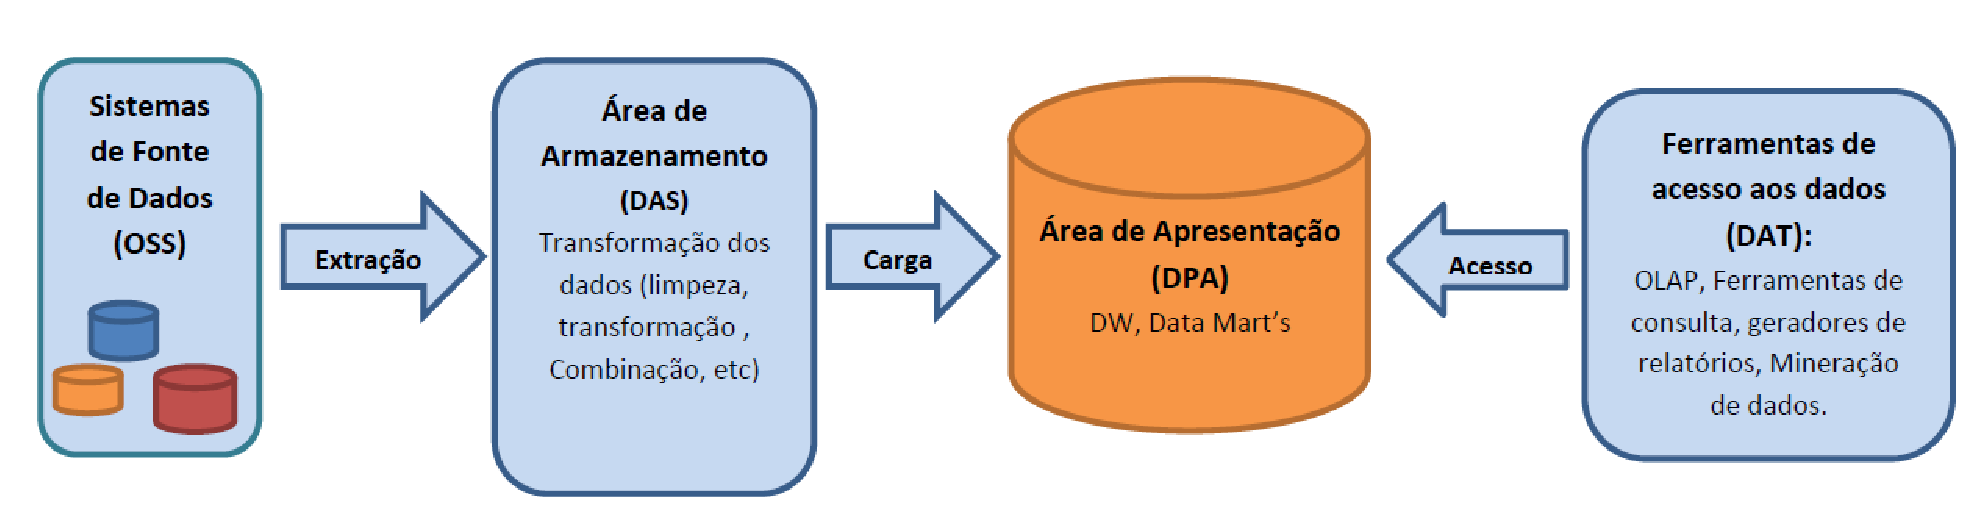
\includegraphics[scale=0.5]{figuras/componentesDW}
 		\caption{Componentes de um \emph{DWing}. Adaptação de \cite{kimball2002}}.
 		\label{componentesdw}
 \end{figure}


%TODO: ver se concorda com o fato de não termos subseções aqui
% a figura acima estava sem explicação/interpretação "explicita"
 A extração dos dados que irão compor o DW é feita de fonte de dados de sistemas, podendo ser de um ou vários sistemas relacionados. Esses dados são tratados na DSA, onde podem ser combinados, limpados ou transformados, tornado-os mais consistentes para que possam então ser amazenados na DPA, que seriam o DW ou \emph{Data Mart's}
 %
 \footnote{\emph{Data Mart} é um subconjunto de dados de um DW. Foca em uma ou mais áreas específicas \cite{kimball2002}}. 
 %
 As ferramentas de acesso são as responsáveis pela análise dos dados, podendo realizar consultas, gerar relatórios entre outros mecanismos de visualização. Cada um dos componentes serão um pouco mais detalhados a baixo, pois revelam algumas características fundamentais de um ambiente de \emph{DWing}.

\begin{description}
	\item[Sistemas de Fonte de Dados Operacionais - OSS]
\end{description}
%

O Sistemas de Fonte de Dados Operacionais (OSS - \emph{Operational Source Systems}) são as fontes dos dados de negócio que irão compor o ambiente de DW.
%
Pode ser de origem de várias aplicações que compõe o sistema corporativo de uma instituição, podendo ser unificada com uma única ou várias bases de dados.
%
Não podem ser consideradas dentro do escopo do \emph{DWing}, pois  não se tem nenhum controle sobre o conteúdo ou sobre o formato de dados provenientes da fonte \cite{kimball2002}.
%
Essas bases de dados não precisam utilizar necessariamente da mesma tecnologia, podendo ser um banco de dados transacionais, arquivos de texto, planilhas, arquivos XML ou qualquer outra forma de se armazenar e representar informações de negócio.

\begin{description}
\item[Área de Preparação dos Dados - DSA]
\end{description}
%

A Área de Preparação dos Dados (DSA - \emph{Data Staging Area}) é o ambiente no qual é feita a extração, transformação e carga dos dados operacionais, processo comumente chamado de ETL (\emph{Extract, Transform, Load}).
%
Essa área de preparação, denominada por Kimball (\citeyear{kimball2002}), utiliza arquivos simples ou tabelas relacionais temporários, não acessíveis aos usuários, para armazenamento e manipulação das informações durante o processo de ETL.
%
Assim que os dados estiverem prontos é feito a carga na base de dados dimensional, base essa acessível ao usuário.
%
A etapa de extração dos dados consiste em ler e entender as fontes de dados e extrair apenas os dados necessários para o DW.
%
Os dados extraidos na camada OSS não são integrados, e, segundo Inmon (\citeyear{inmon2002}), esses dados, dessa forma, não podem ser utilizados para dar suporte a uma visão corporativa, que é uma das essências do ambiente de \emph{DWing}.
%
Dessa forma, uma série de transformações podem ser feitas buscando a limpeza de dados (resolução de conflitos, tratamento de informações não existente, conversão de dados para um formato padronizado), combinação de dados de diversas fontes, remoção de dados duplicados e atribuições de chaves que serão utilizadas no DW \cite{kimball2002}.
%
Ao final da transformação, as informações necessárias são selecionadas e incluídas na base de dados multidimensional, encontrada na área de apresentação que será tratada em seguida.

\begin{description}
\item[Área de Apresentação - DPA]
\end{description}
%

A Área de Apresentação dos dados (DPA - \emph{Data Presentation Area}) é onde os dados são organizados, armazenados e disponibilizados para consultas á usuários ou ferramentas de geração de relatórios ou análises. Esse ambiente pode ser materializado no DW em si \cite{kimball2002}. 


Um dos principais propósitos de um DW é ter uma navegação intuitiva e de alta performance \cite{kimball2002}. A visualização das informações de um DW é resultado de agregações de dados, ou seja, diferentes formas de agrupamentos de dados que geram diferentes tipos de informações. Essas agregações são caracterizadas pelas consultas OLAP. Dessa forma, a modelagem relacional, normalmente utilizadas em bancos de dados transacionais, não dão suporte esses propósitos, pois a base de dados é normalizada e a agregação de grande número de dados torna-se custosa em termos de performance. O processo de normalização foi inicialmente proposto por Byce Codd  que consiste em esquematizar as relações de uma base de dados relacional, minimizando redundância de informações e anomalias de inserção, exclusão e alteração, no que diz respeito a manter a consistência de dados caso haja a duplicidade deste. Dessa forma, uma base de dados relacional normalizada oferece mais segurança em transações de acesso e alteração/inclusão/deleção de dados pois possui esquemas menores e consistentes \cite{elmasri2006}. O problema de esquemas menores é a performance, pois a realização consultas exige a navegação  entre várias tabelas, e se tratando de uma consulta que envolve grande quantidades de dados, como em um \emph{DWing}, a performance se torna um fator muito importante para a qualidade do ambiente.

Kimball (\citeyear{kimball2002}) então propõe o uso da modelagem dimensional, que possui as mesmas informações que as bases normalizadas, porém em um formato diferente, atendendo a facilidade na navegação e na performance das consultas. Mais detalhamento sobre a modelagem dimensional será vista na Seção (\ref{sec-dimensional-modeling}).

\begin{description}
\item[Ferramentas de Acesso de dados – Visualização de dados:]
\end{description}

As Ferramentas de Acesso a Dados são ferramentas que tem a capacidade de realizar consulta aos dados da Área de Apresentação. Elas podem variar desde simples ferramentas de consulta \emph{ad-hoc} até ferramentas de análises complexas e de mineração de dados \cite{kimball2002}.

Ferramentas de visualização são muito importantes em um ambiente de \emph{DWing}, pois são essas ferramentas que irão facilitar o acesso a informação coletada, que é o primeiro requisito de um abiente de \emph{DWing} listado por Kimball (\citeyear{kimball2002}). Um dos modos de se apresentar os dados é através de relatórios, que são vistas agregadas da informação que sejam relevantes para a tomada de decisão. Muitas ferramentas permitem a realização de consultas OLAP \emph{ad-hoc} para a criação de relatórios customizados ou até mesmo a definição de relatórios definidos que são utilizados com frequência. A partir desses relatórios podem ser extraídos gráficos, sendo este mais um meio de facilitar a visualização da informação. 
%TODO: Achei as explicações acima muito longas. Tentar ser mais objetivo, uma vez que agora estamos usando tais descrições para explicar a figura citada acima.
%Carlos: Acredito que tais descrições são necessárias pois revelam algumas caracteríticas importantes do DW que são tratadas em cada componente, como a preocupação com a performance, redundancia entre outros aspectos. Fiz uma descrição breve da figura e fiz um link para os detalhes, ok?

Outra forma de visualização de dados é dada através  de \emph{dashboards}, que são muito úteis para o monitoramento de indicadores por ser basicamente uma tela com informações resumidas com diferentes elementos de exploração como tabelas, graficos, manometros, entre outros.
%TODO: acho que não precisa de figura e explicação sobre dashboard (pelo menos da forma como está)
%TODO: ver se concorda em retirarmos/comentarmos
%Carlos: eu acho que seria interessante falar sobre dashboards pois é um mecanismos de visualização que pode ser muito útil para o monitoramento


\subsection{Modelagem dimensional}
\label{sec-dimensional-modeling}

%TODO: Fazer uma introduççao falando o pq da modelagem dimensional no DW, pq q é importante
A modelagem dimensional é uma tecnica que define bem um ambiente de DW. Segundo Kimball \citeyear{kimball2002} a modelagem dimensional é a única técnica viável para banco de dados  que devem responder a consultas em um DW.

A modelagem dimensional é mais simples, mais expressiva e mais fácil de compreender do que a modelagem relacional \cite{ballard1998}. A modelagem dimensional busca obter um modelo que representa um conjunto de medidas que são descritas por aspectos comuns de negócio.
%
Os conceitos básicos da modelagem dimensional são:

\begin{itemize}
	\item \textbf{fatos}: são dados que contém medidas e seu contexto. Cada fato pode representar uma transação do negócio ou um evento que pode ser usado para análise do próprio negócio. São instâncias da realidade  que podem ser mensuradas de maneira quantitativa \cite{kimball2002}. Em um DW os fatos são armazenadas em tabelas de fatos, que consomem cerca de 90\% do espaço de uma base de dados dimensional. Tabela de fatos é a principal tabela de um modelo dimensional \cite{kimball2002,ballard1998}.

	\item \textbf{dimensões}: determinam os detalhes do contexto em que foi obtido um fato. São tabelas que contem as descrições textuais de negócio e ajudam na identificação de um componente da respectiva dimensão. Cada fato se relaciona com várias dimensões, associado a apenas a um dado em cada uma dessas dimensões.

	\item \textbf{medidas}: é um atributo numérico do fato. A medida determina a performance ou o comportamento de aspectos do negócio. As medidas são determinadas como combinações de membros de dimensões e alocados na tabela de fatos.
\end{itemize}

%TODO: recomenda-se que a figura apareça antes dela ser citada no texto.
%... mudei aqui

 \begin{figure}[!htb]
 	\centering
 		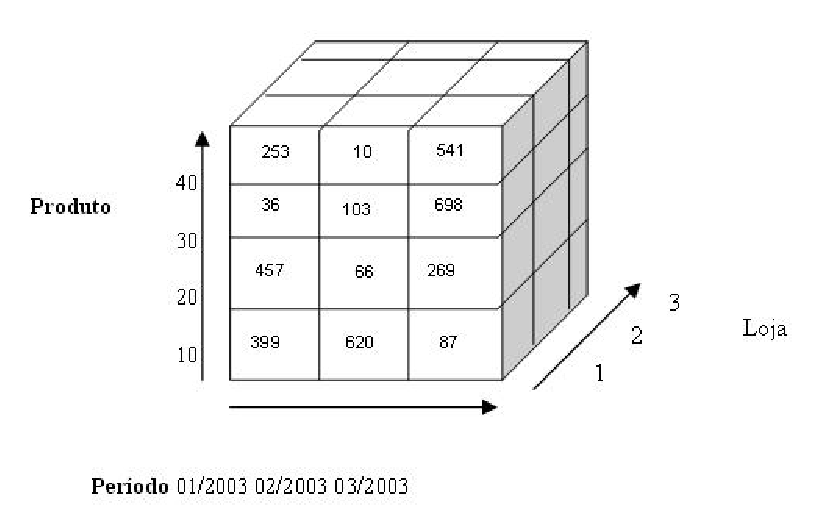
\includegraphics[scale=0.8]{figuras/dw-cubo}
 		\caption{Exemplo de cubo de dados Fonte: \cite{Guimaraes2012}}.
 		\label{dw-cube}
 \end{figure}

A ideia da modelagem dimensional é representar os tipos de dados de negócio em estruturas de cubo de dados. As células desse cubo contém os valores medidos e os lados definem as dimensões. Na Figura \ref{dw-cube} é exemplificado um cubo de dados para o contexto de uma loja. As células desse cubo pode representar a quantidade de vendas, sendo possível a realização de diferentes análises.

 \begin{figure}[!htb]
 	\centering
 		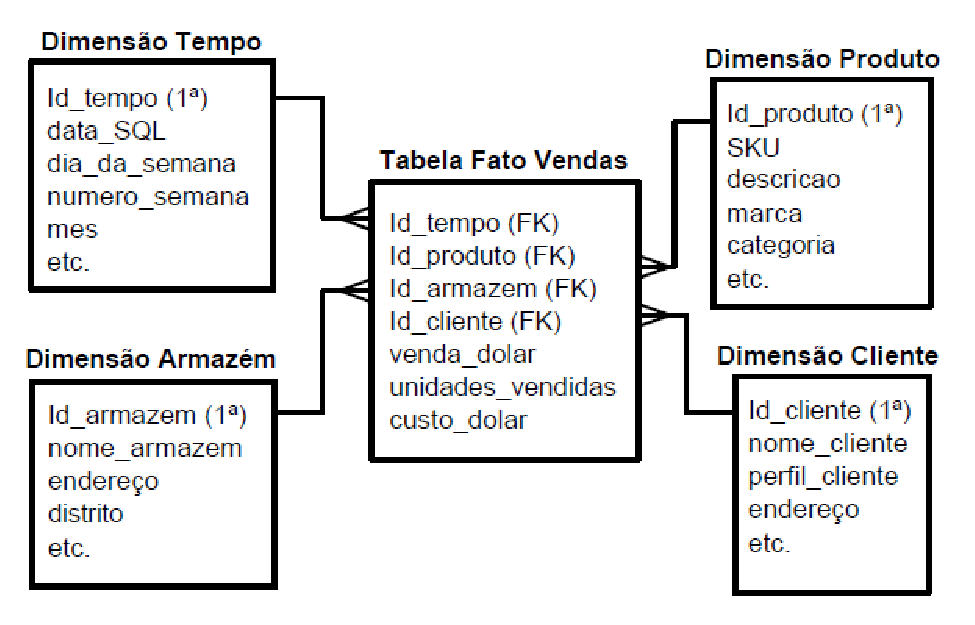
\includegraphics[scale=0.8]{figuras/dw-Modelo-estrela}
 		\caption{Esquema estrela Fonte: \cite{Wagner2012}}.
 		\label{dw-starscheme}
 \end{figure}

O modelo dimensional proposto por Kimball (\citeyear{kimball2002}) é chamado de modelo estrela (\emph{star scheme}, Figura \ref{dw-starscheme}). Nele, temos a tabela fato no centro e varias tabelas dimensões se relacionando com essa tabela fato. As tabelas fatos devem possuir duas ou mais chaves estrangeiras para as chaves primárias de diferentes dimensões. Para juntar as informações basta realizar um \emph{Join} entre elas.
%
Uma Tabela de Dimensão deve ser construída de maneira a incluir atributos que podem ser agregados, fornecendo ao usuário maneiras alternativas de visualizar as informações. No contexto desse trabalho, essa característica nos permite analisar, por exemplo, quais os métodos com mais vulnerabilidades e subir o nível de hieraquia, agregando os dados para visualizar as classes com mais vulnerabilidades, os pacotes, projetos, e assim por diante. Diferente do modelo relacional, o fato da tabela dimensão não ser normalizada implica na melhoria da performance, pois nesse exemplo citado, “Classe” do método normalmente seria outra tabela, e para a referida análise seria necessário a realização de um \emph{Join}, que foi substituído apenas por uma clausula \emph{Group by}.

\begin{figure}[!htb]
 	\centering
 		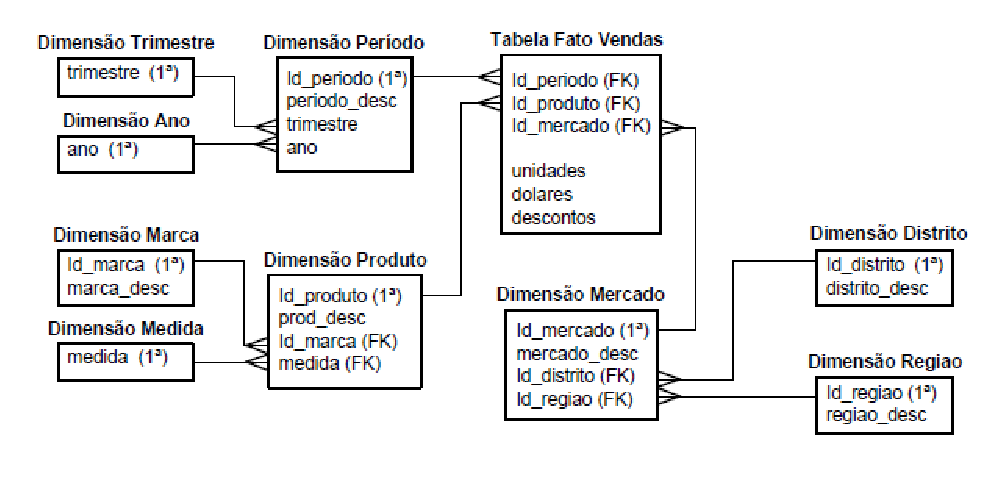
\includegraphics[scale=1]{figuras/dw-modelo-flocodeneve}
 		\caption{Esquema floco de neve  Fonte: \cite{Wagner2012}}.
 		\label{dw-snowflackscheme}
 \end{figure}
%TODO: as figuras estão sem referencia (essa e outras)

Porém, tabelas dimensões podem ser normalizadas com o intuito de diminuir o uso do espaço de armazenamento de informações redundantes \cite{kimball2002}. Nesse caso, quando uma dimensão é normalizada passa-se a ter o esquema floco de neve, como pode ser visto na Figura \ref{dw-snowflackscheme}. Esse esquema torna mais fácil a manutenção de dimensões, porém é aconselhado o seu uso apenas em situações que realmente seja necessário abrir mão da performance que o esquema estrela oferece.
%
A modelagem dimensional facilita o processamento analítico dos dados (OLAP), aspecto que será tratado na Seção \ref{sec-olap}.
%
Kimbal (\citeyear{kimball2002}) define quatro passos que guiam o processo da modelagem dimensional, que são:

 \begin{itemize}

 	\item \textbf{Selecionar o processo de negócio a ser modelado}: consiste em definir qual o assunto no qual o \emph{DWing} será orientado. Como ja foi explicado, o DW é orientado a assunto, e tomando como exemplo um sistema de vendas de uma loja, pode ser feita a análise sobre as vendas, sobre o estoque, etc. Selecionar o processo de negócio é selecionar qual desses assuntos serão analizados e modelados.

 	\item \textbf{Declarar o \emph{"grão"} do processo de negócio}: significa especificar exatamente o que uma linha da tabela de fatos representa. Nessa etapa é definido o nível de glanuralidade da informação. Por exemplo, visualizar as informações por dia ou por mês. A granularidade se refere ao nível de detalhe que o fato deve ter. 

 	\item \textbf{Escolher as dimensões}: consiste em definir as dimensões que se aplicam acada linha de fato que foi definido. Se o nível granularidade foi bem definido, é fácil definir as dimensões. 

 	\item \textbf{Identificar fatos}: consite em responder a pergunta \"o que estamos medindo?\". Nessa estapa é definido os fatos numéricos que irão popular as tabelas fatos.	  
 \end{itemize}

\subsection{OLAP}

\label{sec-olap}

O Processamento Analítico \emph{On-Line} (OLAP – \emph{On-line Analytc Processing}) é toda atividade de consulta que busca trazer ao usuário uma visão analítica dos dados através de comparações, visões personalizadas, análises históricas, diferentes cenários e entre outras opções \cite{kimball2002}.
%
Pode-se definir OLAP como sistemas ou ferramentas que realizam consultas ao DW.
%
Tais sistemas permitem aumentar ou diminuir o nível de detalhes da informação através das operações descritas abaixo. 

 %\begin{figure}[!htb]
 %	\centering
 %		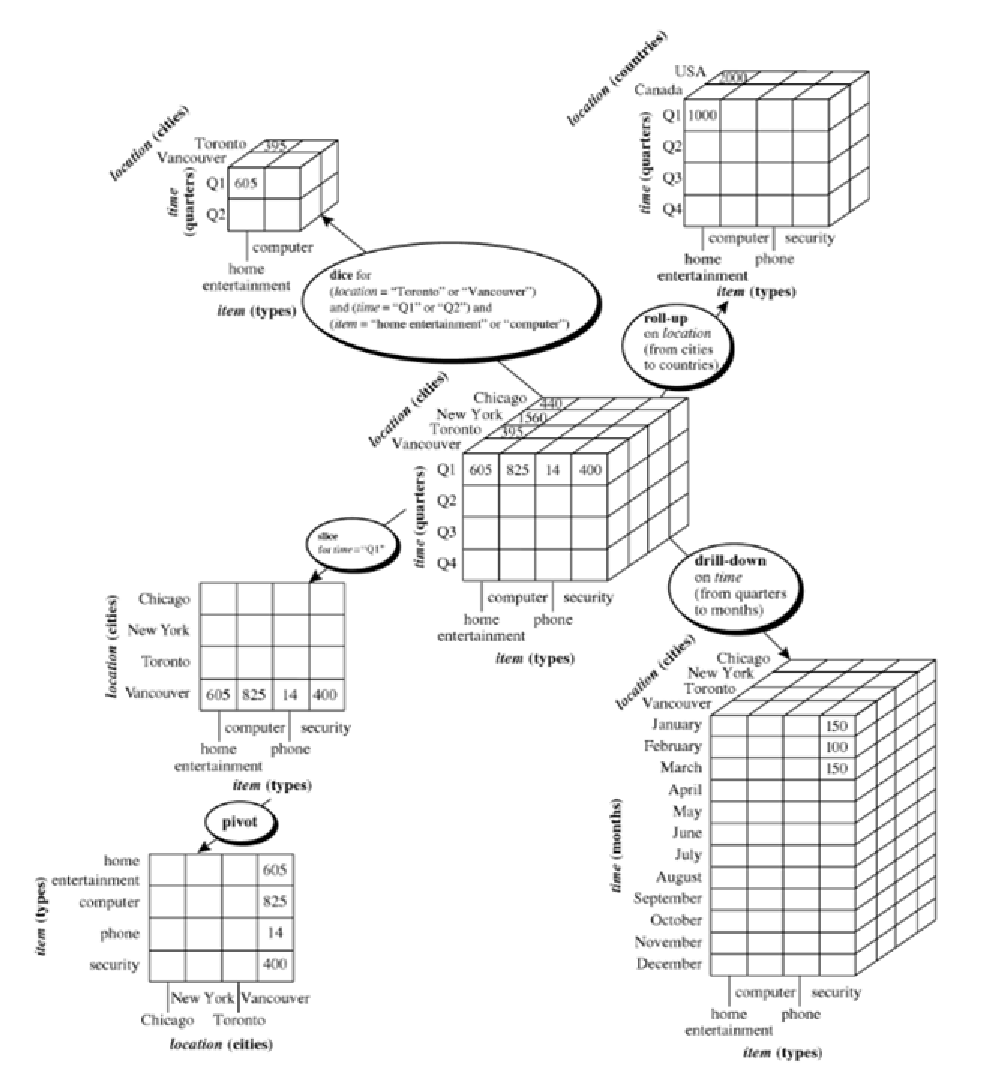
\includegraphics[scale=1]{figuras/olap}
 %		\caption{Operações OLAP}.
 %		\label{dw-olap}
 %\end{figure}
%TODO: esta figura está ruim de ler no pdf. Melhorar ou repensar o uso dela para o TCC 2.


\begin{itemize}

	\item \textbf{\emph{Drill down}}: Consiste em navegar em uma informação de menor nível de detalhe para uma informação de maior nível de detalhe. Por exemplo, uma análise utilizando a dimensão tempo fornece o tempo por bimestre. Uma operação de \emph{Drill Down} consistiria em trazer essa mesma informação por mês. Este exemplo pode ser visto na Figura \ref{fig-dw-rollup}.
\end{itemize}
	
\begin{figure}[!htb]
 	\centering
 		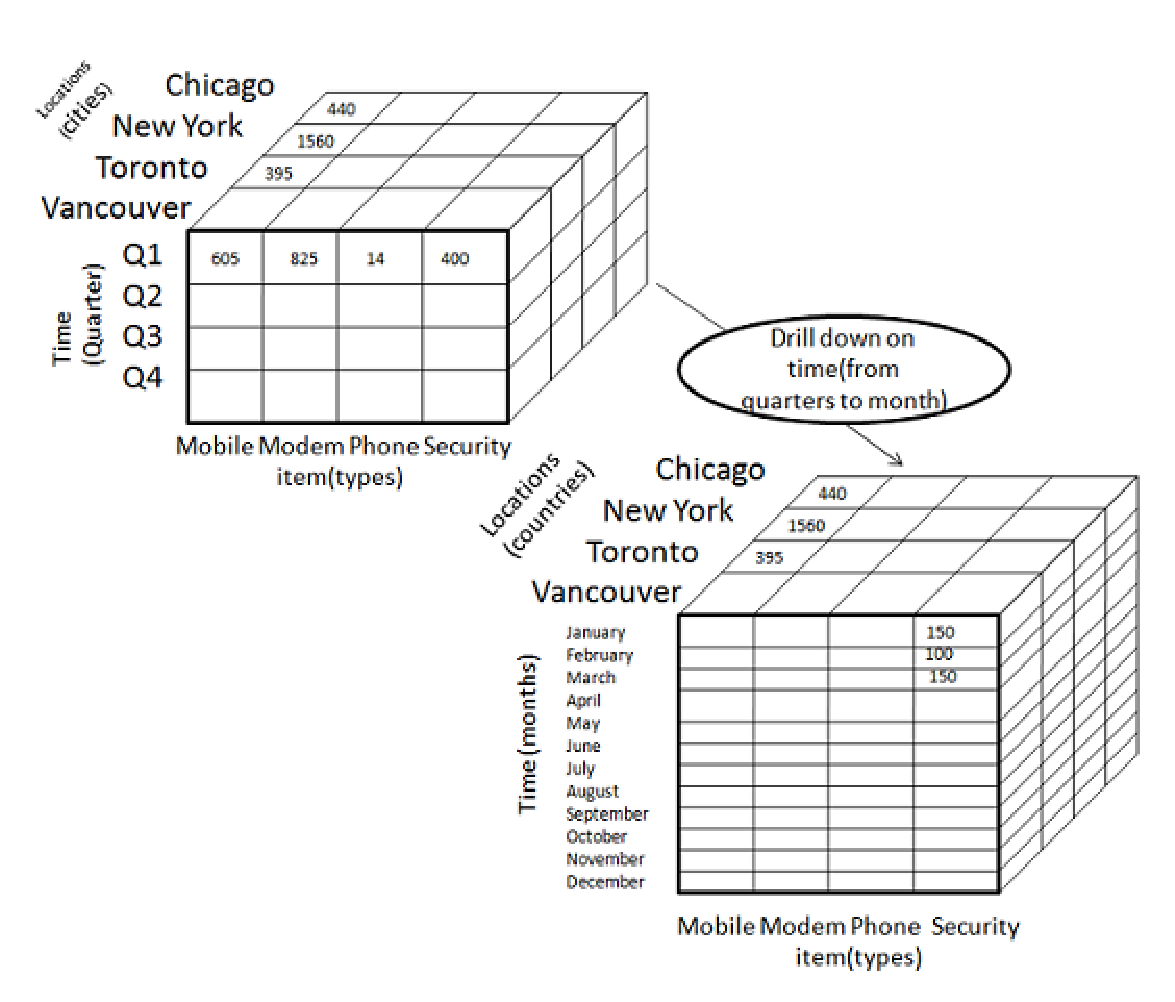
\includegraphics[scale=0.7]{figuras/dw-drill-down}
 		\caption{Demonstração da operação de \emph{Drill Down}   Fonte: \cite{TutorialsPoint}}
 		\label{fig-dw-rollup}
 \end{figure}

\begin{itemize}
	\item \textbf{\emph{Roll up}}: Consiste em navegar em uma informação de maior nível de detalhe para um menor nível de detalhes. É exatamente o inverso do \emph{Drill down}.
 \end{itemize}

 %\begin{figure}[!htb]
 %	\centering
 %		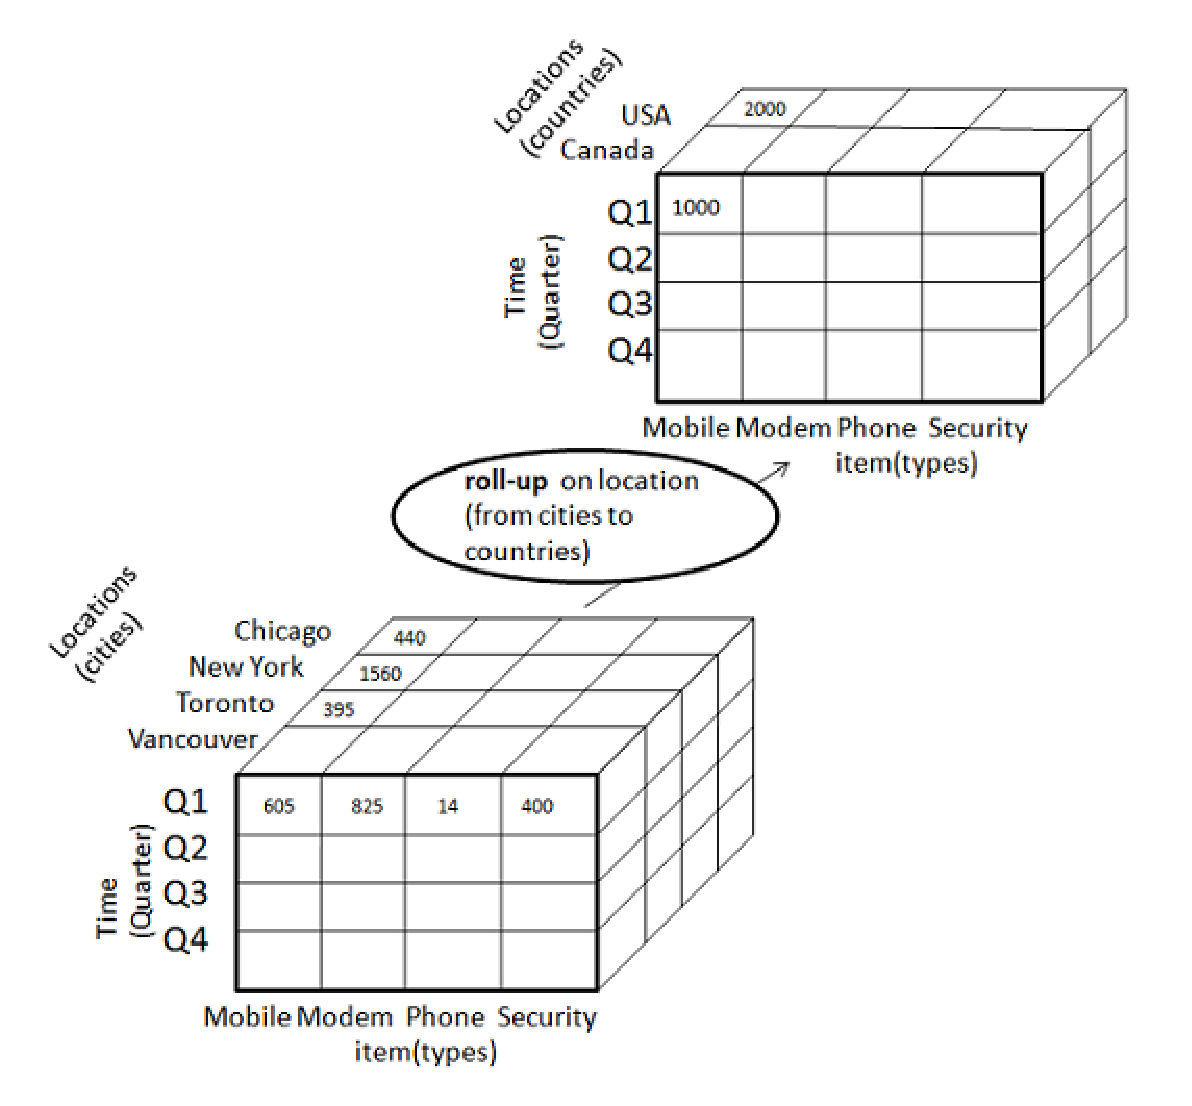
\includegraphics[scale=1]{figuras/dw-rollup}
 %		\caption{Demonstração da operação de Roll up    Fonte: TutorialsPoint}.
 %		\label{dw-rollup}
 %\end{figure}

\begin{itemize}
	\item \textbf{\emph{Slice and dice}}: A operação de \emph{slice} consiste em fatiar o cubo, que consiste em selecionar um atributo de uma dimensão específica e olhar apenas as informações das outras dimensões sobre esse atributo, eliminando a dimensão fatiada. Por exemplo, dado o cubo demosntrado na Figura \ref{fig-dw-slice}, a operação \emph{slice} foi feita ao selecionar apenas as informações do primeiro bimestre (Q1), eliminando qualquer outra informação da dimensão de tempo. A operação \emph{dice}, como o nome sugere, consiste em fatiar em formato de cubo. Nessa caso, não será eliminado nenhuma dimensão, mas será selecionado alguns subgrupos em duas ou mais dimensões, resultando em um subcubo. Por exemplo,  a operação de \emph{dice} no cubo representado na Figura \ref{fig-dw-dice} consistiu em selecionar apenas as informações de Toronto ou Vancouver, no primeiro e segundo bimestre e de apenas itens Mobile ou Modem, gerando um subcubo menor.
\end{itemize}

 \begin{figure}[!htb]
 	\centering
 		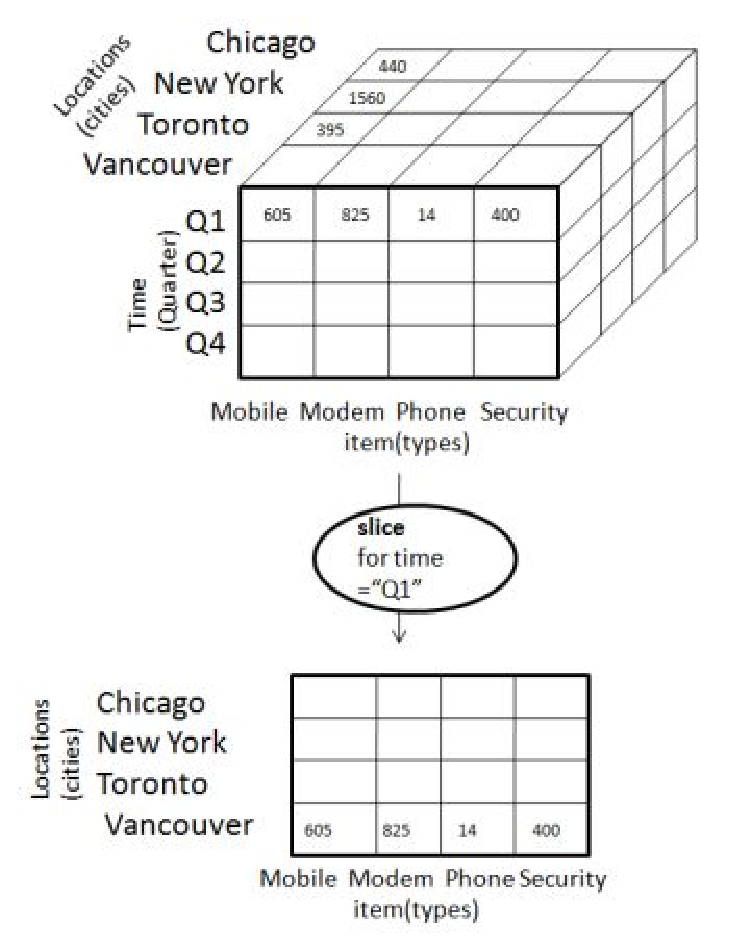
\includegraphics[scale=0.7]{figuras/dw-slice}
 		\caption{Demonstração da operação de \emph{Slice}    Fonte: \cite{TutorialsPoint}}
 		\label{fig-dw-slice}
 \end{figure}

\vspace{10cm}
 \begin{figure}[!htb]
 	\centering
 		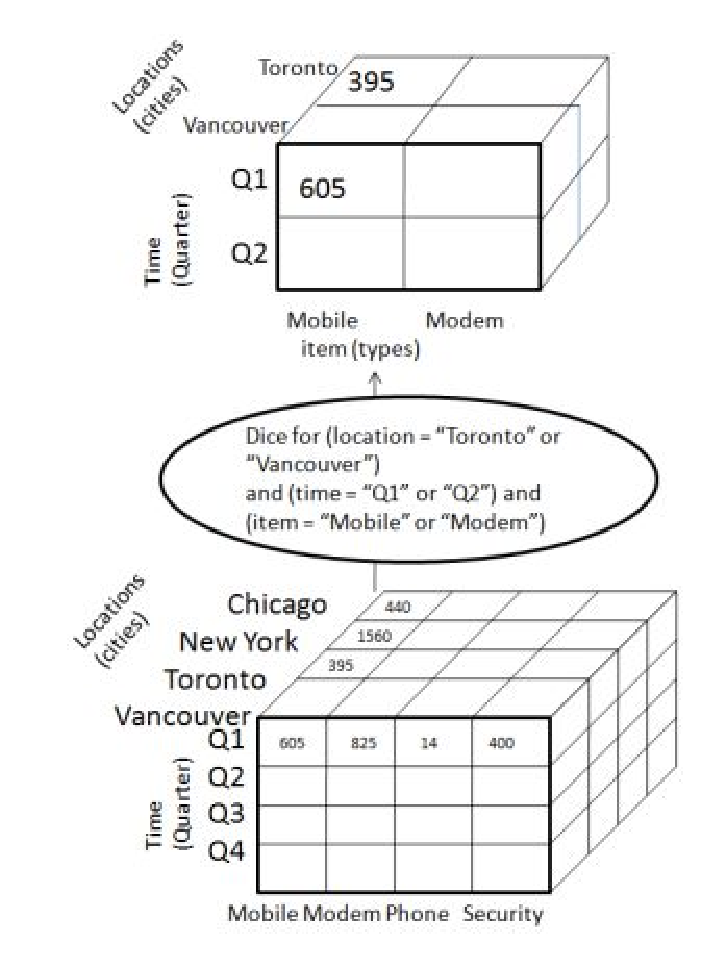
\includegraphics[scale=0.7]{figuras/dw-dice}
 		\caption{Demonstração da operação de \emph{Dice}    Fonte: \cite{TutorialsPoint}}
 		\label{fig-dw-dice}
 \end{figure}
\begin{itemize}


 \begin{figure}[!htb]
 	\centering
 		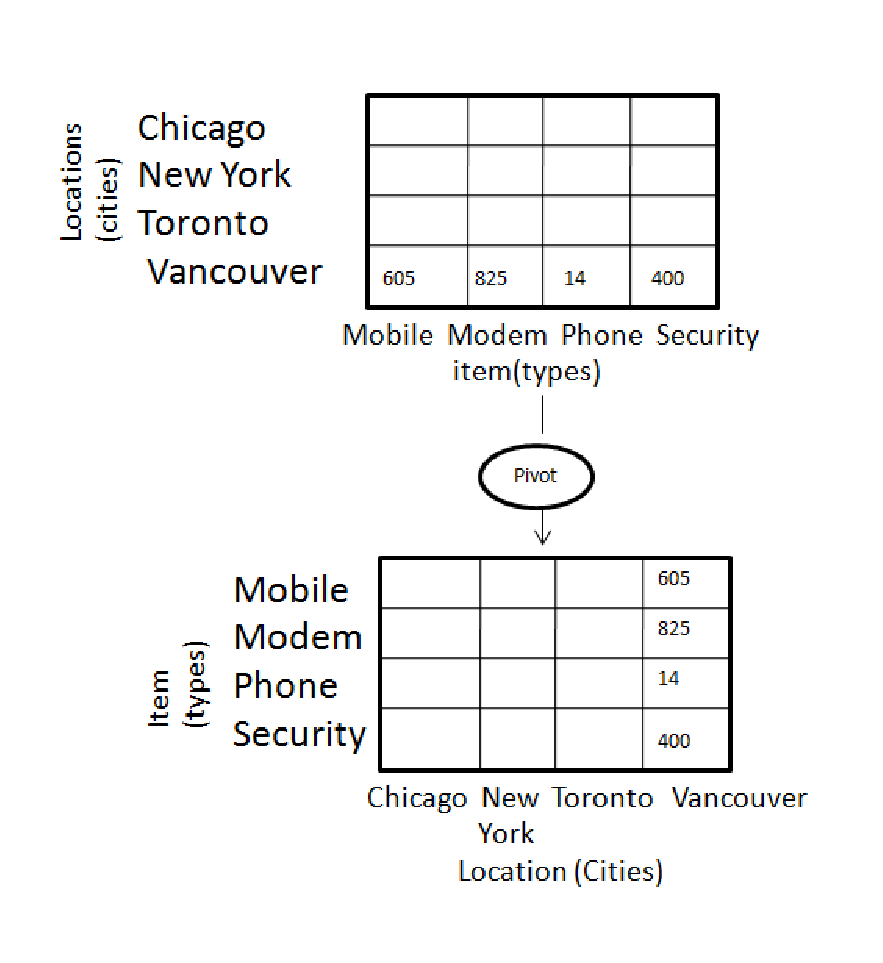
\includegraphics[scale=0.55]{figuras/dw-pivot}
 		\caption{Demonstração da operação de \emph{Pivoting}    Fonte: \cite{TutorialsPoint}}
 		\label{fig-dw-pivot}
 \end{figure}

	\item \textbf{\emph{Pivoting}}: Também conhecida como \emph{rotate}, é uma operação que realiza uma rotação nos eixos de um cubo, gerando uma visualização alternativa da informação \cite{cavalcanti2012}. O resultado de uma operação de \emph{pivoting} pode ser visto na Figura \ref{fig-dw-pivot}.  
\end{itemize}
 




\subsection{Ciclo de vida de um ambiente de \emph{Data Warehousing}}
\label{sec-lifecycleDw}

Kimball (\citeyear{kimball2002}) define um ciclo de vida para o processo de construção de um ambiente de \emph{DWing}. Neste ciclo, a primeira atividade a ser realizada é o planejamento do projeto. Essa atividade consiste em avaliar a iniciativa de construção do \emph{DWing}, estabelecendo um escopo inicial e a justificativa, como também contempla a obtenção  de recursos e o lançamento do projeto.

 \begin{figure}[!htb]
 	\centering
 		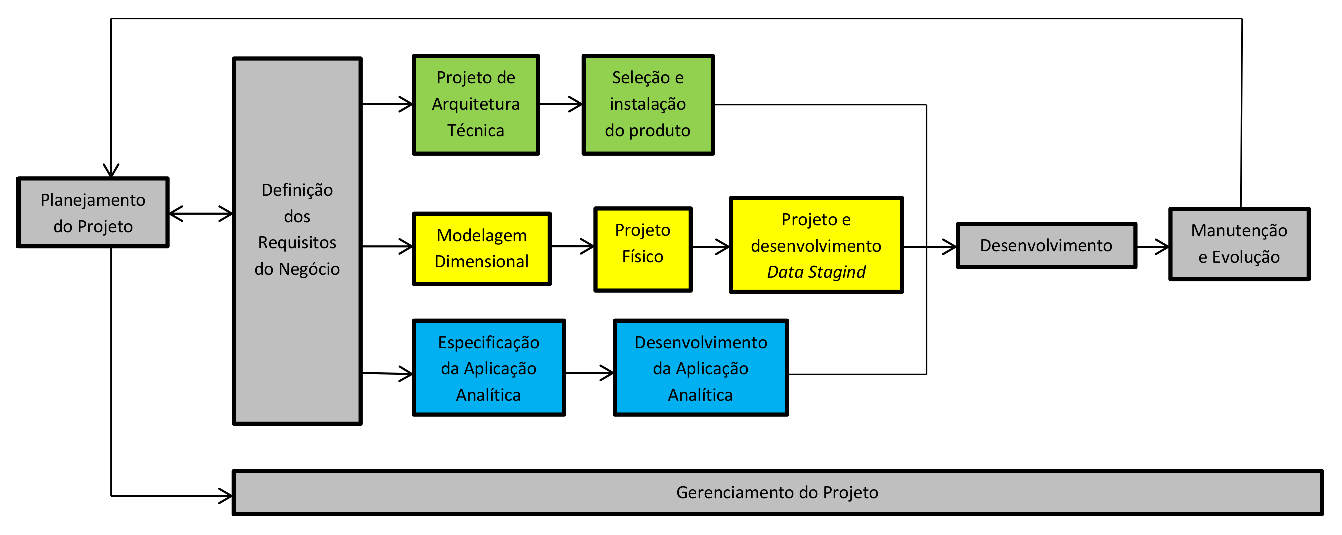
\includegraphics[scale=0.7]{figuras/dw-ciclo-de-vida}
 		\caption{Ciclo de vida de um Projeto de \emph{DWing} \cite{kimball2002}}.
 		\label{dw-lifecycle}
 \end{figure}

A próxima atividade é a definição dos requisitos de negócio. O alinhamento do \emph{DWing} com o s requisitos dos usuários é absolutamente crucial. Não adianta construir o ambiente com as melhores ferramentas do mercado se o este não fornece a informação que o usuário precisa ver. Dessa forma, mais de 50\% das iniciativas de \emph{DWing} não tem sucesso \cite{sen2011}. Pelo levantamento feito na pesquisa de Kimpel (\citeyear{kimpel2013}), a principal causa é o não entendimento do problema que o usuário de negócio quer solucionar. E é na etapa de requisitos que o problema e as necessidades devem ser entendidos e transformados em requisitos de negócio para as etapas seguintes, de modelagem e construção do ambiente.

%

Com os requisitos definidos, existem três conjuntos de tarefas. As tarefas superiores (na cor verde) da Figura \ref{dw-lifecycle} são responsáveis pela concepção tecnológica do ambiente. Consiste na definição da arquitetura técnica e  seleção das tecnologias envolvidas na solução de \emph{DWing}. O conjunto de tarefas que se encontram no meio do ciclo (na cor amarela) são responsáveis pelo desenho do modelo dimensional e físico e a definição e desenvolvimento do processo de ETL dos dados. O conjunto de tarefas inferiores (na cor  azul) são responáveis pelo desenho e desenvolvimento das aplicações analíticas, que irão fornecer a visualização da informação gerada pela \emph{DWing} para o usuário. Juntando esses três conjuntos de tarefas temos a implantação e disponibilização do ambiente de \emph{DWing} para o usuário, então pode-se dizer que a solução de \emph{DWing} foi implantada e pode começar a ser utilizada. 


No fim do ciclo ainda existe uma atividade de manutenção e crescimento do ambiente, dado que esse é um tipo de ambiente que deve evoluir dinamicamente de acordo com o negócio e suas necessidades de tomada de decisão.


\subsection{Construção de ambiente de DW para o monitoramento de métricas de software.}

%

Nas seções anteriores foi feito uma revisão teórica sobre as principais caracteríticas de um ambiente de \emph{DWing}. Neste trabalho, buscamos desenvolver um ambiente de \emph{DWing} que auxilie no monitoramento e na tomada de decisão, baseado em métricas de software. Dessa forma, a proposta é desenvolver um ambiente que nos permita coletar métricas de ferramentas de análise estática de código, identificar o cenários de decisão a partir da correlação dessas métricas (assunto que será abordado no Capítulo \ref{cap-cenarios}) e sugerir refatorações para solucionar esse cenário. A suíte de ferramentas Analizo, como fornecedor de métricas, irá compor o componente OSS da arquitetura de um \emph{DWing} discutida no inícío desta seção. O Pentaho é uma suíte de ferramentas de BI que oferece desde mecanismos de ETL, \emph{reporting}, OLAP e mineração de dados. Essa ferramenta nos permitirá extraír, tratar e analisar os dados de relatórios do Analizo a fim de identificar os cenários de decisão. Os recursos OLAP irão permitir diferentes visões que permitirá identificar diversas características que poderão auxiliar na tomada de decisão, como qual a classe que possui mais cenários, qual cenário é o mais recorrente, além de poder extrair indicadores a partir dos dados e analisar o histórico das informações, verificando se houve melhoria ou não na situação do projeto.

Percebe-se que vários recursos de um ambiente de \emph{DWing} podem ser explorados a fim de dar mais informações a respeito de um projeto de software a partir de métricas. Entretanto, tais aspéctos e configurações da solução serão ainda  definidos e refinados para a composição da solução final.

%

%TODO: Não achei didático este capítulo/texto sobre DW. Foi muito "mais do mesmo" sem contextualizar, exemplificar e casar com o trabalho em si.
%TODO: Para o TCC 2 ser mais objetivo e contextualizar as explicações com o trabalho, ou seja, ser mais didático e simples.
%TODO: observem que ao terminar este capítulo a pergunta que fica é "e aí? o que farei isso mesmo?"

